\documentclass{article}
\usepackage[utf8]{inputenc}

\usepackage{float}
\usepackage{natbib}
\usepackage{graphicx}
\usepackage[export]{adjustbox}
\usepackage{multirow}
\usepackage{hyperref}
\usepackage{titlesec}
\usepackage{ragged2e}


\documentclass{article}
\usepackage{bera}% optional: just to have a nice mono-spaced font
\usepackage{listings}
\usepackage{xcolor}

\colorlet{punct}{red!60!black}
\definecolor{background}{HTML}{EEEEEE}
\definecolor{delim}{RGB}{20,105,176}
\colorlet{numb}{magenta!60!black}

\lstdefinelanguage{json}{
    basicstyle=\normalfont\ttfamily,
    numbers=left,
    numberstyle=\scriptsize,
    stepnumber=1,
    numbersep=8pt,
    showstringspaces=false,
    breaklines=true,
    frame=lines,
    backgroundcolor=\color{background},
    literate=
     *{0}{{{\color{numb}0}}}{1}
      {1}{{{\color{numb}1}}}{1}
      {2}{{{\color{numb}2}}}{1}
      {3}{{{\color{numb}3}}}{1}
      {4}{{{\color{numb}4}}}{1}
      {5}{{{\color{numb}5}}}{1}
      {6}{{{\color{numb}6}}}{1}
      {7}{{{\color{numb}7}}}{1}
      {8}{{{\color{numb}8}}}{1}
      {9}{{{\color{numb}9}}}{1}
      {:}{{{\color{punct}{:}}}}{1}
      {,}{{{\color{punct}{,}}}}{1}
      {\{}{{{\color{delim}{\{}}}}{1}
      {\}}{{{\color{delim}{\}}}}}{1}
      {[}{{{\color{delim}{[}}}}{1}
      {]}{{{\color{delim}{]}}}}{1},
}




\begin{document}
\title{COS301 Team Gamma: Pushing to Github}
\begin{figure}
    \centering
    
\includegraphics[width=\textwidth]{logo.png}
\end{figure}
\date{Draft - March 2020}

\maketitle

\section{Introduction}
This document describes the methodology in how to manage our Github repository.

\newpage

\section{Github Structure}
\subsection{General details}
Since our student package accounts cannot create Github organisations - we are required to create a single repository and add everyone as collaborators. \\

The repository is up at: \url{https://github.com/gjcsup/cos301_teamgamma} \\

You will be added to the Github repository as a collaborator.

\subsection{Branching Structure}
\begin{figure}[h]
    \centering
    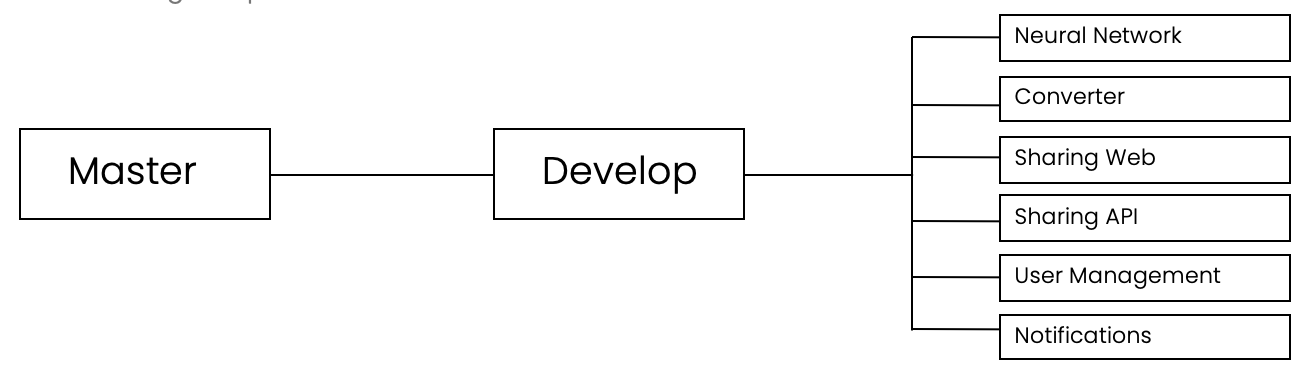
\includegraphics[width=\textwidth]{branches.png}
\end{figure}

\vspace{0.5cm}

Each team will work on their own branch that will merge into a develop branch.

\begin{center}
\textbf{ALWAYS INSURE THAT YOU ARE WORKING ON YOUR TEAM'S BRANCH.}
\end{center}
\newline
\begin{center}
   \textit{Further detail will be added in revisions of this document.}
\end{center}

\newpage
\subsection{Folder structure}
\begin{itemize}
\item \textbf{app}
    \begin{itemize}
    \item Specific sub structure to be determined (read more below)
    \end{itemize}
\item \textbf{database}
    \begin{itemize}
    \item sharing
    \item usermanagement
    \end{itemize}
\item \textbf{documentation}
    \begin{itemize}
    \item androidfrontend
    \item converter
    \item integration
    \item neuralnetwork
    \item notification
    \item sharing
    \item usermanagement
    \item webfrontend
    \end{itemize}
\item \textbf{server}
    \begin{itemize}
    \item sharing
    \item usermanagement
    \item neuralnetwork
    \end{itemize}
\end{itemize}

\newpage

\section{Description of Directories}
\subsection{app}
The Flutter files will be stored and organised underneath this directory. This will be the directory that has the most concurrent teams working on it.\\
\newline
\textbf{Teams that work here:}
\begin{itemize}
    \item Android Frontend (Integration team)
    \item Converter
    \item Neural Network
    \item Notification
\end{itemize}

\subsection{database}
The Database .sql files will be stored and organised in this directory. Other teams won't be interacting with the database as everything happens through the actual deployed API. \\
\newline
\textbf{Teams that work here:}
\begin{itemize}
    \item UserManagementAPI
    \item SharingAPI
\end{itemize}

\subsection{documentation}
Each team's Overleaf .tex and output .pdf files will be stored and organised in this directory. Each team works in their own subdirectory. \\
\newline
\textbf{Teams that work here:}
\begin{itemize}
    \item Everyone
\end{itemize}

\newpage
\subsection{server}
All files running on external servers will be organised here (PHP files etc). Each API team works in their own subdirectory. Sometimes another team will make changes to your code, such as Notification adding functions to SharingAPI. \\
\newline
\textbf{Teams that work here:}
\begin{itemize}
    \item UserManagementAPI
    \item SharingAPI
    \item Notification
    \item Neural Network
    \item WebFrontend
\end{itemize}

\section{What to push for Demo \#1}
\subsection{Important Notice}
Each team working in the /app directory is going to be working separately for demo \#1 as we are merely showing the direction in which we are working. This will cause merge conflicts. Our solution is to move all of these "prototypes" to a aptly named sub-folder \textbf{after} Friday before we merge and start working coherently for the next phase.

\begin{center}
\textbf{THERE WILL BE NO MERGE FOR DEMO \#1.}
\end{center}

\subsection{All Teams:}
\begin{itemize}
    \item Documentation (Download all the files (images, main.tex etc) from Overleaf) to /documentation/teamname directory
\end{itemize}

\subsection{'/app' Directory Teams:}
\begin{itemize}
    \item All your flutter code to the /app directory (using your own sub-directory structure, preferably the default as setup by Flutter) 
\end{itemize}

\subsection{'/database' Directory Teams:}
\textit{Command to export database: mysqldump -u [username] -p [databaseName] > filename.sql}
\begin{itemize}
    \item The .sql export file to the /database/teamname directory
\end{itemize}

\subsection{'/server' Directory Teams:}
\begin{itemize}
    \item The .php file to /server/teamname
    \item NeuralNetwork team - whatever you guys have to upload here (if anything), also in /server/teamname
\end{itemize}

\subsection{Notification Team:}
\begin{itemize}
    \item Your .php file to /server/teamname
    \item Your Flutter files to /app
\end{itemize}

\end{document}